\documentclass{beamer}

\mode<presentation>
\setbeamerfont{footnote}{size=\tiny}
\setbeamertemplate{navigation symbols}{}

\usetheme{Warsaw}

\usepackage[backend=bibtex,style=verbose]{biblatex}
\usepackage{graphicx}

\usepackage{tikz}
\usetikzlibrary{backgrounds,positioning,fit}
\usepackage{adjustbox}
\usepackage{mathtools}
\usepackage{xcolor}
\DeclarePairedDelimiter{\norm}{\lVert}{\rVert}

\usepackage[linesnumbered,lined,noline,ruled,noend]{algorithm2e}
\usepackage{subfig}
\usepackage{pgfplots}

\AtBeginSection[]
{
	\begin{frame}
		\frametitle{Outline}
		\tableofcontents[currentsection]
	\end{frame}
}

\bibliography{./bibs/Asynchronous-Applications,./bibs/Asynchronous-FT,./bibs/Asynchronous-Theoretical,./bibs/Example-Problems,./bibs/Fault-Tolerance,./bibs/Fixed-Point,./bibs/General-HPC,./bibs/HPC-Math-Software,./bibs/Iterative-Methods,./bibs/Preconditioning,./bibs/Self-Citations,./bibs/Textbooks}

\title[Randomized Asynchronous Linear Solvers]{Dynamic Non-Uniform Randomization in Asynchronous Linear Solvers}
\author[Coleman \& Sosonkina]{Evan Coleman\inst{1} \and Masha Sosonkina\inst{2}}

\institute % (optional)
{
  \inst{1}%
  United State Department of Defense
   \and
  \inst{2}%
  Old Dominion University\\
}
\date{$17^{\rm th}$ Copper Mountain Conference on
Iterative Methods\\ April 4--8, 2022}

\begin{document}

%------------------------------------------------------------------------------
% Front matter
%
\begin{frame}
	\titlepage
\end{frame}


\begin{frame}
	\frametitle{Outline}
	\tableofcontents
\end{frame}

\section{Motivation}

\begin{frame}
	\frametitle{Introduction}
	\begin{itemize}
		\item Problem: solve the linear system $Ax = b$
		\item Some systems don't need to be solved with high accuracy
		    \begin{itemize}
		        \item e.g., in AI applications arriving quickly at a sufficiently good answer is preferable to waiting longer for a highly accurate answer
		    \end{itemize}
		\item Asynchronous solvers gain prominence at the exascale and heterogeneous systems.
	    \item There are a number of papers that explore the feasibility of using randomized linear solvers to achieve this goal:
	        \begin{itemize}
	            \item \textcite{leventhal2010randomized}; 
	            $\bullet$ \textcite{griebel2012greedy};
	            $\bullet$ \textcite{avron2015revisiting}
	        \end{itemize}
	\end{itemize}	
\end{frame}

%\begin{frame}
%	\frametitle{Introduction}
%	\begin{itemize}
%		\item Some applications have 
%		\item Some systems don't need to be solved exactly
%		    \begin{itemize}
%		        \item e.g., there may be applications where quickly arriving at a sufficiently good answer is preferable to getting an exact answer in a longer period of time
%		    \end{itemize}
%	    \item There are a number of papers that explore the feasibility of using randomized linear solvers to achieve this goal:
%	\end{itemize}	
%\end{frame}

\begin{frame}
	\frametitle{Motivation}
	\begin{itemize}
		\item \textcite{wolfson2017distributed} investigated  a Southwell-like approach for solving linear systems to improve on Gauss-Scieldel iteration
	\end{itemize}	
	\begin{block}{Question:}
	    Is there a way to combine the natural greediness of the Southwell algorithm with the randomized asynchronous nature of the solvers as proposed in [1--3]?
	\end{block}
\end{frame}


\section{Ideas Under Consideration}

\begin{frame}
	\frametitle{Setting the stage}
	\begin{itemize}
		\item Although these solvers have applications inside other solvers, we focus on their ability to solve systems directly
        \item First we will describe our approach and motivation
        \item Then we'll go over some results and discuss paths forward
	\end{itemize}
\end{frame}

\begin{frame}
	\frametitle{Residual data for finite-difference of 2D Laplacian}
	\begin{figure}[H]
		\centering
		\subfloat[Unsorted residuals]{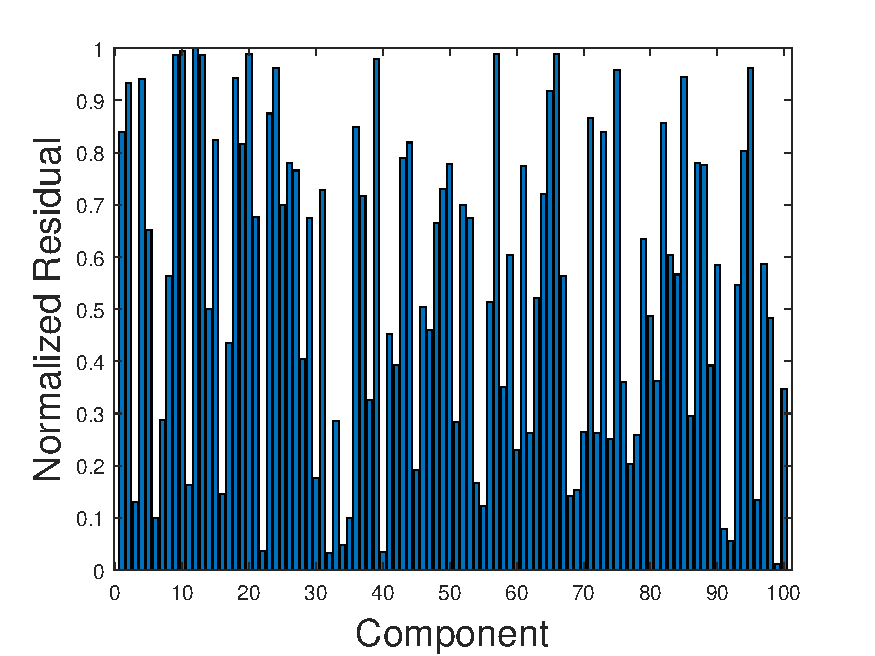
\includegraphics[width=0.50\textwidth]{images/init_resids_10x10.pdf}}
		\subfloat[Sorted residuals]{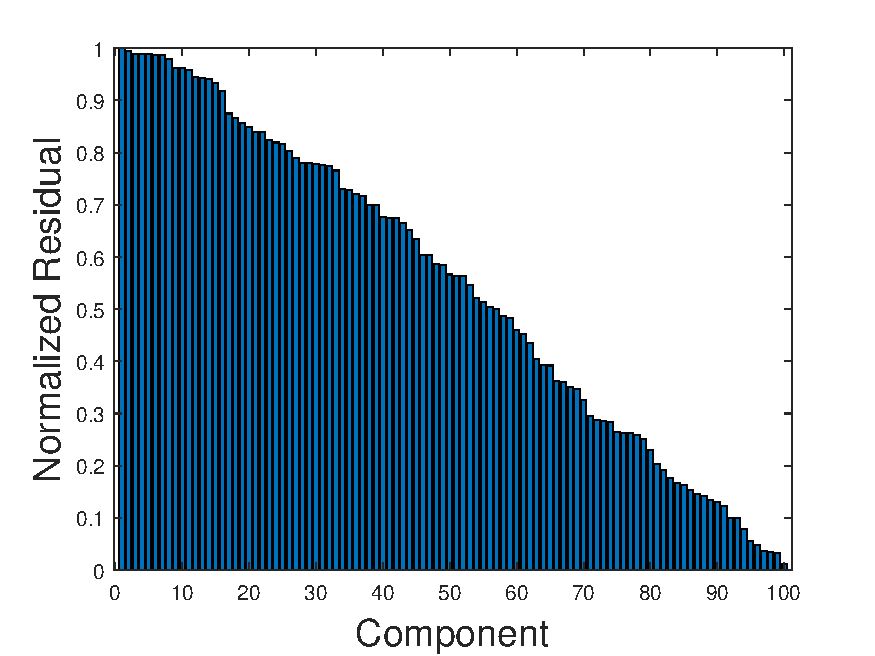
\includegraphics[width=0.50\textwidth]{images/init_resids_10x10_sorted.pdf}}
		\caption{Initial component residuals ($r_i / \max (r_i)$).}
		\label{fig:initial-residuals-laplacian}
	\end{figure}
\end{frame}

% TODO: Add a triangular distribution?
% TODO: Show the distribution at several iteration counts?
% TODO: Find a way to show the comparison with which components would be selected discrete local residual distribution vs discrete diagonal element distribution
\begin{frame}
	\frametitle{Ranked residual data for finite-difference of 2D Laplacian}
	\begin{figure}[H]
		\centering
		\subfloat[Sorted Residuals, exponential distributions]{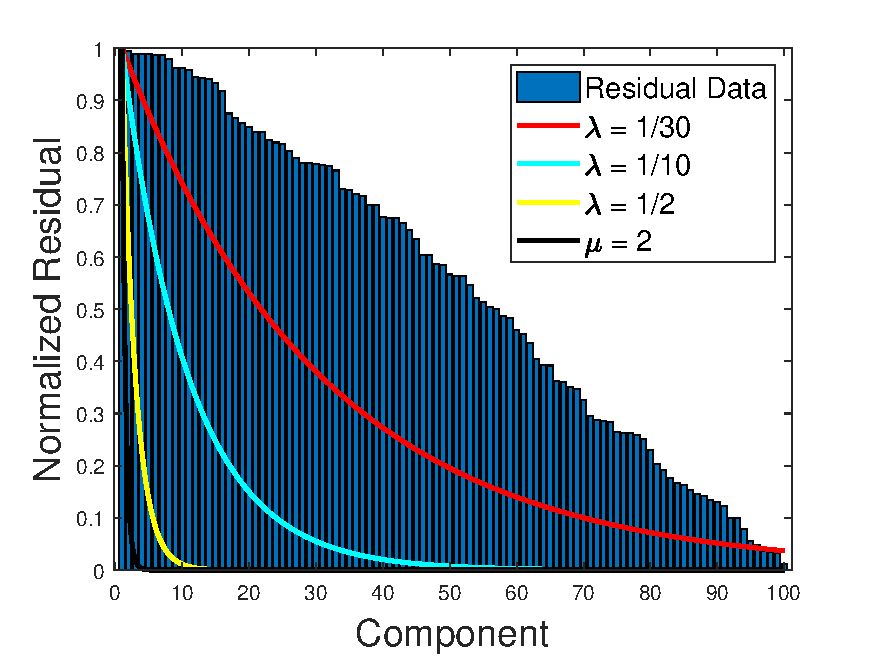
\includegraphics[width=0.75\textwidth]{images/exp_dist_overlay_init.pdf}}
	\end{figure}
\end{frame}


% TODO: Try to clarify/summarize our prior contribution
% TODO: e.g., how does our approach differ from the existing work (Avron & Chow)
\begin{frame}
	\frametitle{Our approach}
	\begin{itemize}
		\item Make the random selection change dynamically 
		\item Goal is to  select the ``right'' residual components (similar to classical Southwell) without the large computational overhead, incurred in the Southwell  by sorting and ranking after each update.
		\item Based around monitoring which (blocks of) residuals contribute most to the residual $r = b - Ax$
		\item Only periodically find and rank the local/component residuals (for the contribution of block $i$):
			\begin{equation}
				r_i = b_i - Ax_i
			\end{equation}
			and make the selection using a {\it non-uniform} distribution that favors selection of components with higher local residual
	\end{itemize}
\end{frame}

\begin{frame}
	\frametitle{Approaches towards making the component selection}
	    \begin{itemize}
	        \item Uniform distribution
	        \item Discrete (non-updated) distribution defined by the ratio of the diagonal element to the trace
	            \begin{equation}
	                \mathbb{P}(i=k) = \frac{a_{kk}}{tr(A)}
	            \end{equation}
	        \item ``Greedy'' selection\footcite{griebel2012greedy} picks an element within a parameter defined threshold of optimal in the Southwell sense 
	    \end{itemize}
\end{frame}


\begin{frame}
	\frametitle{Approaches towards making the component selection}
	    \begin{itemize}
	        \item Discrete distribution defined by the ratio of the local residual to the sum of all residuals
	            \begin{equation}
	                \mathbb{P}(i=k) = \frac{r_{k}}{\sum_j r_j}
	            \end{equation}
	        \item Periodically fitting a continuous distribution to the (sorted) local residuals and drawing random numbers from this distribution
	            \begin{itemize}
	                \item Exponential, triangular
	            \end{itemize}
	    \end{itemize}
\end{frame}

\section{Numerical Results}

\begin{frame}
	\frametitle{More motivation}
	\begin{itemize}
		\item One of the first questions should be: how different are the local contributions to the residual?
		\item For matrices where the local residuals, $r_i$, are similar, any Southwell-like weighting will not show much improvement over a uniform random distribution
	\end{itemize}
\end{frame}


\begin{frame}
	\frametitle{Solver data (Laplacian)}
	\begin{figure}[H]
		\centering
		\subfloat[2D problem (5-pt stencil, $10\times 10$ grid)]{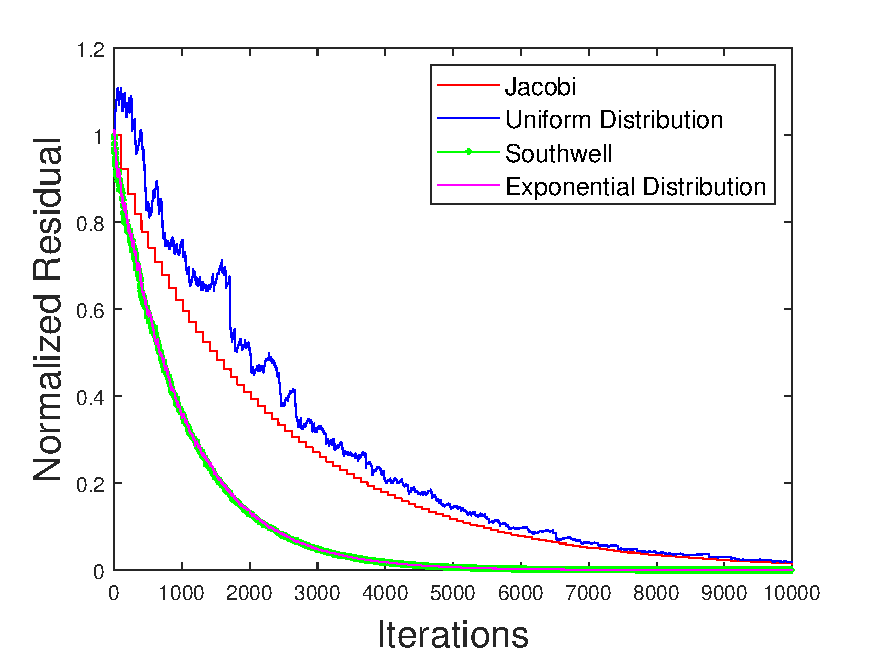
\includegraphics[width=0.45\textwidth]{images/res_10x10.pdf}}
		\subfloat[3D problem (27-pt stencil, $10 \times 10 \times 10$ grid)]{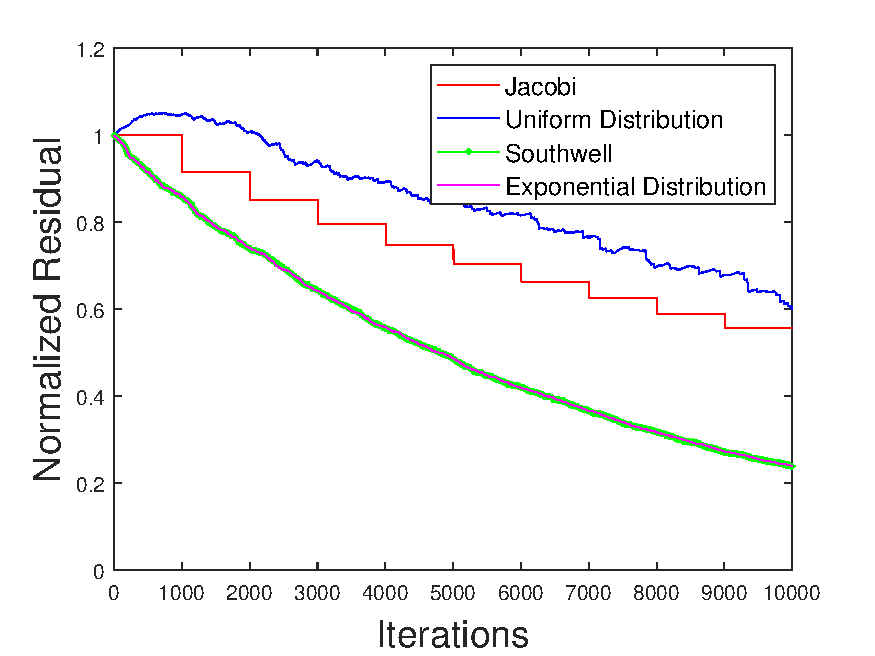
\includegraphics[width=0.45\textwidth]{images/res_3D_10x10x10.pdf}}
		\caption{Residual ($r / r_0$) progression for the first 10,000 iterations of four stationary methods solving the 2D (a) and 3D (b) Laplacian.}
	\end{figure}
\end{frame}

% TODO: Find data (MATLAB or other) showing residual progression of solver methods on another problem
% \begin{frame}
% 	\frametitle{Solver data}
%         \begin{figure}[H]
%         	\centering
%         	\subfloat[Exponential distribution]{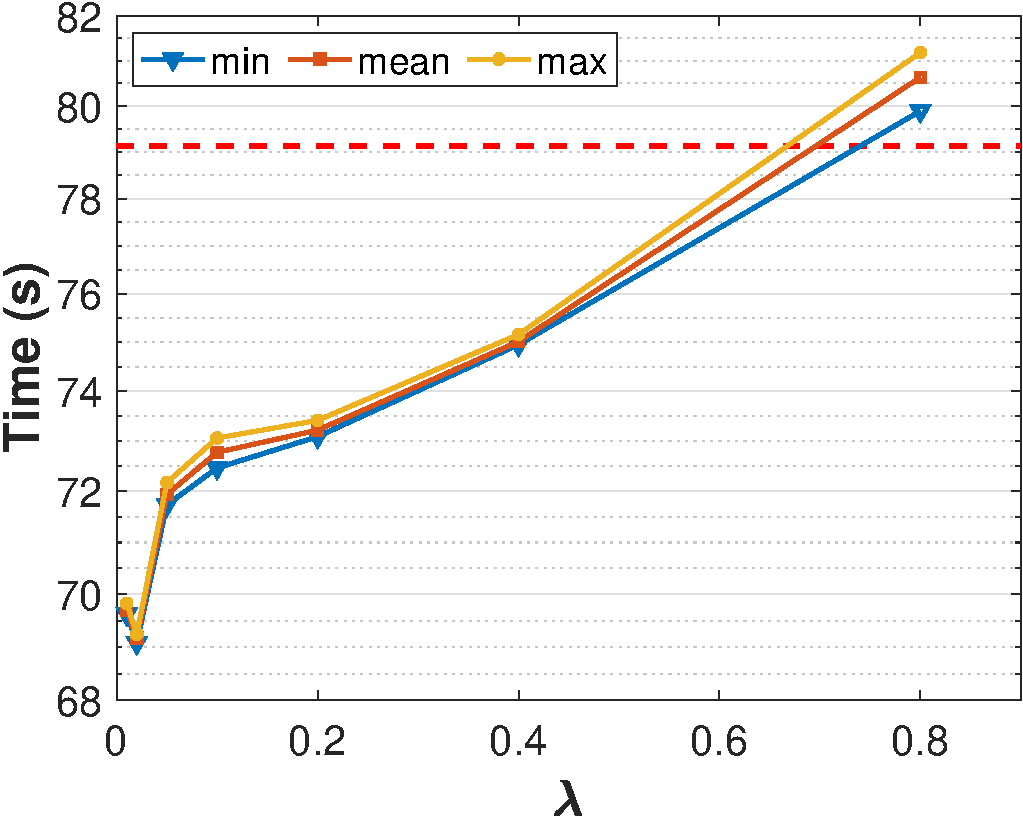
\includegraphics[width=0.75\linewidth]{images/expoDist_calcTimes_all_1tbr.pdf}}
%         \end{figure}
% \end{frame}

\begin{frame}
	\frametitle{Solver data}
       \begin{columns}
          \column{0.5\linewidth}
             \centering
             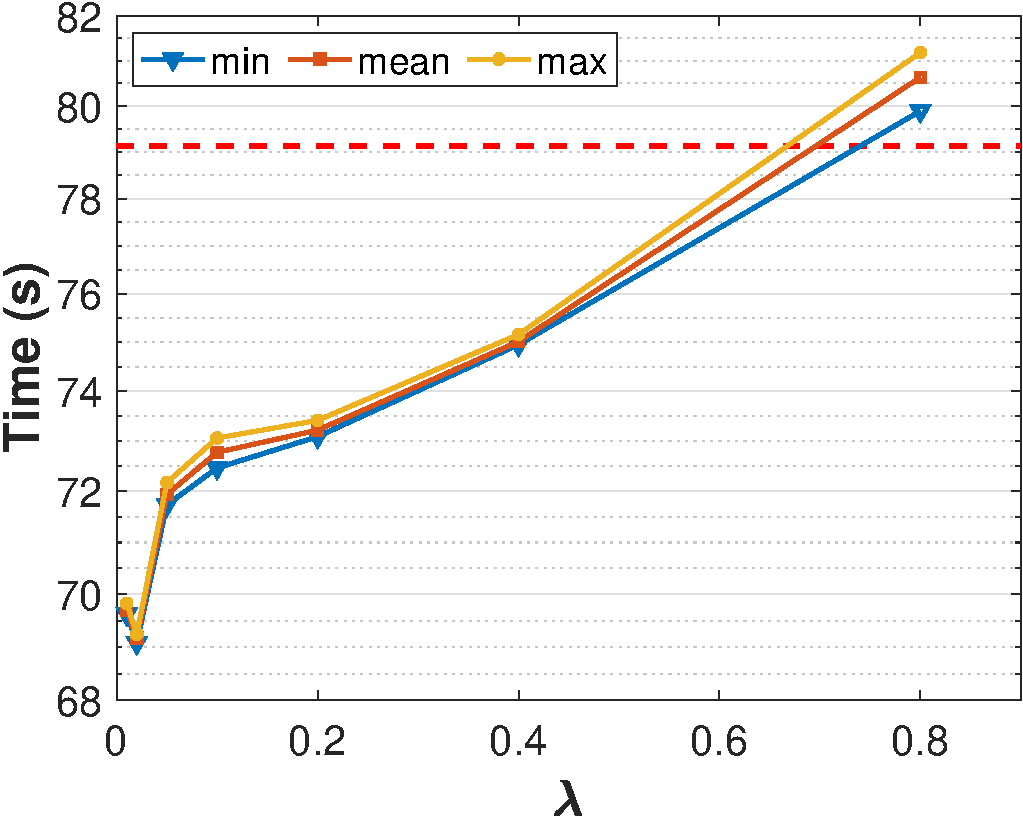
\includegraphics[width=\linewidth]{images/expoDist_calcTimes_all_1tbr.pdf}
           \column{0.5\linewidth}
              \begin{itemize}
                  \item Shared memory experiments on the Rulfo system at Old Dominion University
                  \item 64 core Intel Xeon Phi
                  \item 2D discretization of the Laplacian over an $800 \times 800$ grid
                  \item Dashed red line represents the performance of uniform selection
              \end{itemize}
         \end{columns}
\end{frame}



% TODO: Find data  showing residual progression of solver methods at scale
% \begin{frame}
% 	\frametitle{Solver data (???)}
% 	\begin{itemize}
% 	    \item TODO 2
% 	\end{itemize}
% \end{frame}

\begin{frame}
	\frametitle{Approach: block methods}
	\begin{itemize}
	    \item One of the next logical steps would be to look into the extension of these ideas to block methods
		\item Divide the domain into $m$ subdomains, $\mathbb{R}^n = \mathbb{R}^{n_1} \times \mathbb{R}^{n_2} \times \cdots \mathbb{R}^{n_m}$, where $n = \sum_i n_i$
		\item Each time a block is selected it performs one or more internal iterations of a stationary solver
	\end{itemize}
\end{frame}

\begin{frame}[shrink]
	\frametitle{Notional block picture}
	\begin{figure}[H]
		\scalebox{1.0}{
			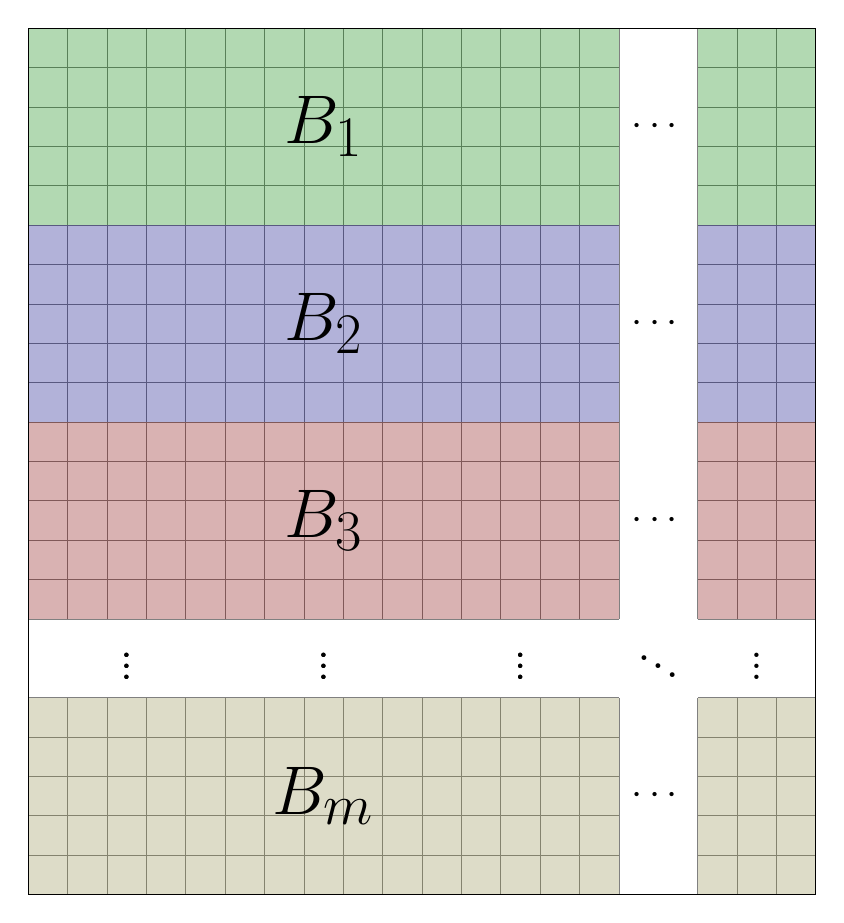
\begin{tikzpicture}
			\draw[step=5mm,gray,very thin] (0,0) grid (7.5,7.5);
			
			\draw[step=5mm,gray,very thin] (0,0) grid (7.5,7.5);
			\draw[step=5mm,gray,very thin] (0,-3.5) grid (7.5,-1);
			
			\draw[step=5mm,gray,very thin] (8.49999,-3.5) grid (10,-1);
			\draw[step=5mm,gray,very thin] (8.49999,0) grid (10,7.5);
			
			\fill[yellow!50!black,opacity=0.3]   (0,-3.5) rectangle (7.5,-1);
			\fill[yellow!50!black,opacity=0.3]   (8.49999,-3.5) rectangle (10,-1);
			
			\fill[green!50!black,opacity=0.3] (0,7.5) rectangle (7.5,5);
			\fill[green!50!black,opacity=0.3] (8.49999,7.5) rectangle (10,5);
			
			\fill[blue!50!black,opacity=0.3]  (0,5) rectangle (7.5,2.5);
			\fill[blue!50!black,opacity=0.3]  (8.49999,5) rectangle (10,2.5);
			
			\fill[red!50!black,opacity=0.3]   (0,2.5) rectangle (7.5,0);
			\fill[red!50!black,opacity=0.3]   (8.49999,2.5) rectangle (10,0);
			
			\node at (8, -2.25) {\bf \Large $\cdots$};
			\node at (8, 1.25) {\bf \Large $\cdots$};
			\node at (8, 3.75) {\bf \Large $\cdots$};
			\node at (8, 6.25) {\bf \Large $\cdots$};
			
			\node at (1.25, -0.5) {\bf $\vdots$};
			\node at (3.75, -0.5) {\bf $\vdots$};
			\node at (6.25, -0.5) {\bf $\vdots$};
			\node at (9.25, -0.5) {\bf $\vdots$};
			
			\node at (8, -0.5) {\bf \large $\ddots$};
			
			\node at (1.25, -0.5) {\bf $\vdots$};
			\node at (3.75, -0.5) {\bf $\vdots$};
			\node at (6.25, -0.5) {\bf $\vdots$};
			
			\node at (3.75, -2.25) {\Huge \bf $B_{m}$};
			\node at (3.75, 1.25) {\Huge \bf $B_3$};
			\node at (3.75, 3.75) {\Huge \bf $B_2$};
			\node at (3.75, 6.25) {\Huge \bf $B_1$};
			
			\draw[black] (0,7.5) rectangle (10,-3.5);
			\end{tikzpicture}
		}
	\end{figure}
\end{frame}

\begin{frame}
	\frametitle{Generic block algorithm}
	\begin{algorithm}[H]
		\DontPrintSemicolon
		\For {each processing element $P_{l}$} {
			\For {$i = 1, 2, \ldots$ until convergence} {
				Pick a block $j \in \{1, 2, \ldots, m\}$ {\em{\underline{somehow}}} \; 
				Read the corresponding entries of $A, x, b$ \;
				Perform Jacobi or Gauss-Seidel relaxations for all equations in block $j$ \;
				Update the data for block $j$ \;
			}
		}
	\end{algorithm}
	\begin{itemize}
	    \item Key: we're performing the dynamic selection on the blocks themselves, and performing traditional iteration inside of the blocks
	\end{itemize}
\end{frame}

\begin{frame}
	\frametitle{Dynamic block algorithm}
	\begin{itemize}
	    \item Instead of dividing the domain into blocks as in the previous image, we create blocks dynamically:
	        \begin{itemize}
	            \item Each thread selects a single row using our selection methodology from before to initialize
	            \item Each update causes each thread to select a new single row using the same methodology
	            \item These two rows create a block where the thread goes throw and performs traditional updates (e.g., Jacobi or Gauss-Seidel) on all components between the two
	        \end{itemize}
        \item Need to add logic to avoid multiple threads trying to write to the same component
	\end{itemize}
\end{frame}

% TODO: Find data  showing residual progression of block solver methods
\begin{frame}
	\frametitle{Solver data from Wahab}
	\begin{figure}
	    \centering
	    \subfloat[Traditional block implementation]{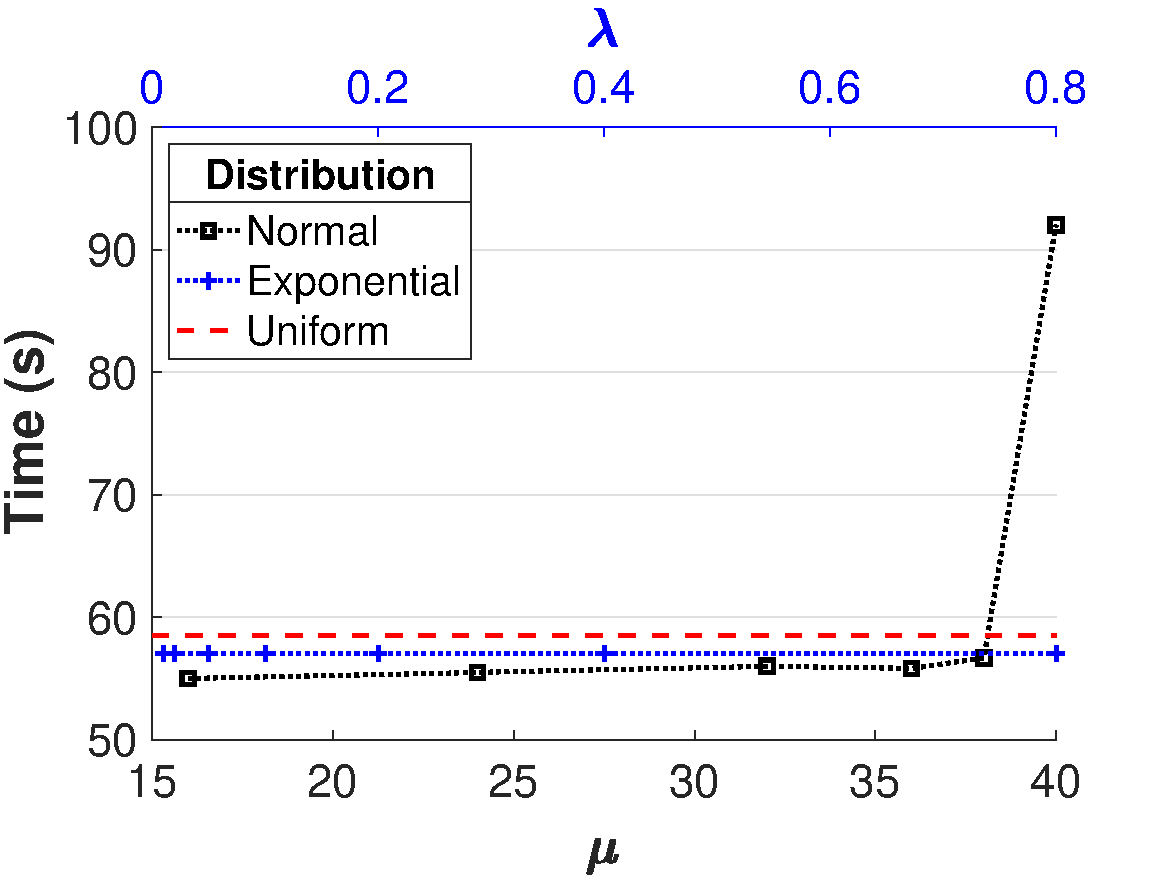
\includegraphics[width=0.5\textwidth]{images/block_time.pdf}}
	    \subfloat[Dynamic block implementation]{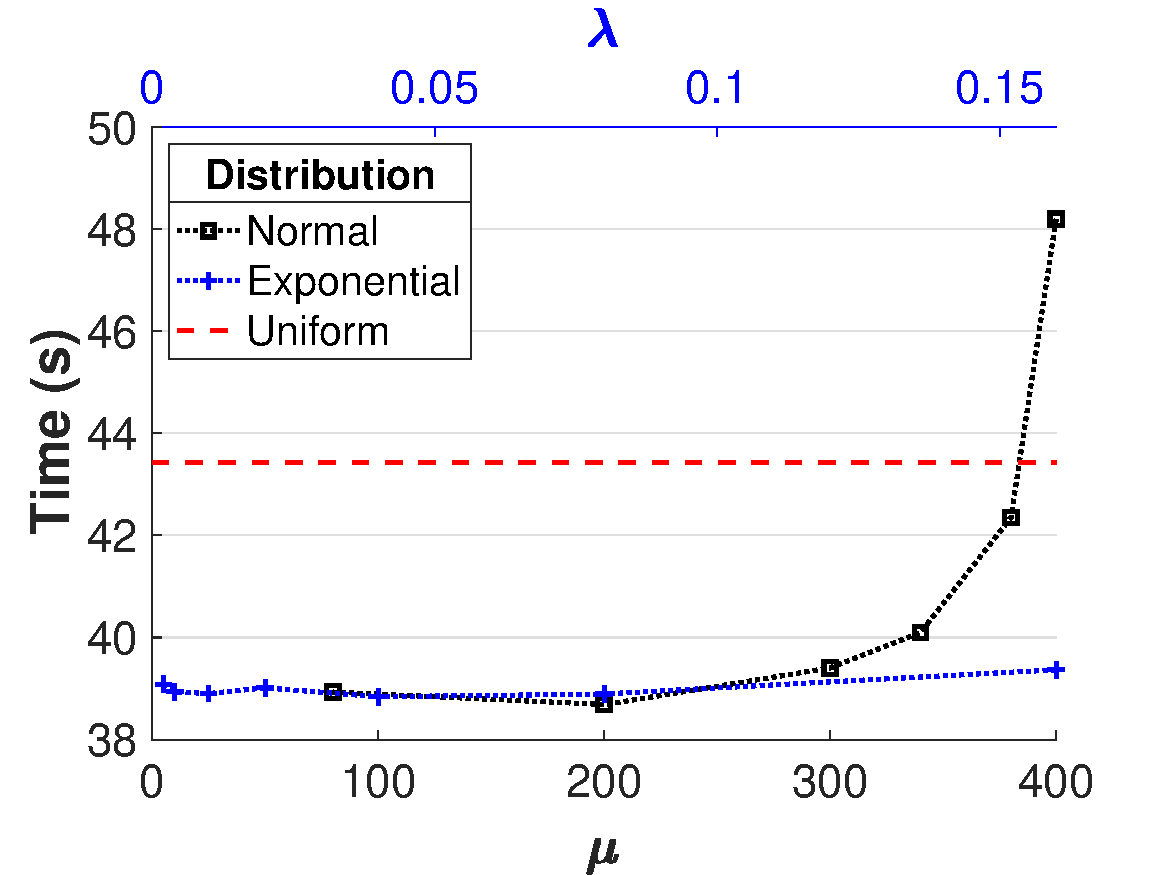
\includegraphics[width=0.5\textwidth]{images/row_time.pdf}}
	\end{figure}
	\begin{itemize}
	    \item Still single node, shared memory experiments (different architecture)
	\end{itemize}
\end{frame}

\section{Summary \& Path Forward}

\begin{frame}
	\frametitle{Summary}
	\begin{itemize}
		\item Dynamic non-uniform randomization provides a potential way to improve the performance of asynchronous linear solvers
		\item Moving forward, many questions need to be answered to establish that it's an area worth pursuing
		\item Initial results do suggest that there is potential for the method to provide a modest improvement over existing techniques in certain circumstances
	\end{itemize}
\end{frame}

\begin{frame}
	\frametitle{Moving forward}
	    \begin{itemize}
	        \item Questions:
	            \begin{itemize}
	                \item How does this extend to a distributed setting?
	                \item How can we optimize some of these parameters based on intrinsic properties of the matrix?
	                \item Does the gain in performance overcome the extra computational overhead?
	            \end{itemize}
	        \item Further investigation:
	            \begin{itemize}
            		\item Try incorporating new solvers into more complex existing routines
            		\item Keep experimenting with different distributions (still chosen beforehand) and ranking methods and periodicities
            		\item Try using an evolving probability distribution where the parameters of distribution shift over time 
	            \end{itemize}
	     \end{itemize}       
\end{frame}
 
\begin{frame}
	\frametitle{}
	\begin{center}
	    Questions? 
	\end{center}
\end{frame}

\begin{frame}
	\frametitle{}
	\begin{center}
	    Back-up
	\end{center}
\end{frame}

\begin{frame}
	\frametitle{Randomized Gauss Seidel (from Avron et al)}
    Let $A \in \mathcal{R}^{n\times n}$ be SPD, $b, x_0 \in \mathcal{R}^n$, then perform iterative updates based on:
        \begin{itemize}
            \item $r_0 = b - Ax_j$
            \item $\gamma_j = d^T_jr_j / d_j^TAd_j$
            \item $x_{j+1} = x_j + \gamma_j d_j$
        \end{itemize}
    for some direction vectors $d_0, d_1, \ldots, d_n$. If the $d_j$ are selected using the distribution,
        \begin{equation}
            Pr(d_j = e_i) = a_{ii} / Tr(A)
        \end{equation}
    then,
        \begin{equation}
            \mathbb{E}[\norm{x_j - x }_A^2] \leq \left( 1 - \frac{\lambda_{min}}{Tr(A)}\right)^m \norm{x_0 - x^*}_A^2
        \end{equation}
\end{frame}

\begin{frame}
	\frametitle{Proof (from Avron's talk in 2013)}
    For simplicity: assume $A$ has unit diagonal via rescaling.
    \begin{enumerate}
        \item $\gamma_j = d_j^Tr_j$
        \item $\norm{x_{j+1} - x}_A^2 = \norm{x_j - x}_A^2 - (d_j^Tr_j)^2$
        \item $\mathbb{E}[(d_j^Tr_j)^2 | r_j] = \frac{1}{n} \norm{r_j}_2^2$
        \item $\lambda_{min} \norm{x_j - x}_A^2 \leq \norm{r_j}_2^2 \leq \lambda_{max} \norm{x_j - x}_A^2$
        \item $\frac{\lambda_{min}}{n}\mathbb{E}[\norm{x_j - x}_A^2] \leq \mathbb{E}[(d_j^Tr_j)^2] \leq \frac{\lambda_{max}}{n}\mathbb{E}[\norm{x_j - x}_A^2]$
    \end{enumerate}
\end{frame}

\begin{frame}
	\frametitle{Randomized Gauss Seidel (new distribution)}
    Let $A \in \mathcal{R}^{n\times n}$ be SPD, $b, x_0 \in \mathcal{R}^n$, then perform iterative updates based on:
        \begin{itemize}
            \item $r_0 = b - Ax_j$
            \item $\gamma_j = d^T_jr_j / d_j^TAd_j$
            \item $x_{j+1} = x_j + \gamma_j d_j$
        \end{itemize}
    for some direction vectors $d_0, d_1, \ldots, d_n$. If the $d_j$ are selected using the distribution,
        \begin{equation}
            Pr(d_j = e_i) = r_{i} / \sum_k r_k
        \end{equation}
    then,
        \begin{equation}
            \mathbb{E}[\norm{x_j - x }_A^2] \leq \left( 1 - \frac{\lambda_{min}}{Tr(A)}\right)^m \norm{x_0 - x^*}_A^2
        \end{equation}
\end{frame}

\begin{frame}
	\frametitle{Proof (adapted)}
    For simplicity: assume $A$ has unit diagonal via rescaling.
    \begin{enumerate}
        \item $\gamma_j = d_j^Tr_j$
        \item $\norm{x_{j+1} - x}_A^2 = \norm{x_j - x}_A^2 - (d_j^Tr_j)^2$
        \item $\mathbb{E}[(d_j^Tr_j)^2 | r_j] \color{red}{\geq}  \color{black} \frac{1}{n} \norm{r_j}_2^2$
        \item $\lambda_{min} \norm{x_j - x}_A^2 \leq \norm{r_j}_2^2 \leq \lambda_{max} \norm{x_j - x}_A^2$
        \item $\frac{\lambda_{min}}{n}\mathbb{E}[\norm{x_j - x}_A^2] \leq \mathbb{E}[(d_j^Tr_j)^2] \leq \frac{\lambda_{max}}{n}\mathbb{E}[\norm{x_j - x}_A^2]$
    \end{enumerate}
\end{frame}



\end{document}